\chapter{ПРОЕКТИРОВАНИЕ МОДЕЛЕЙ КОМБИНАЦИОННОЙ ЛОГИЧЕСКОЙ СХЕМЫ}

\section {Постановка задачи}
Спроектировать синтезируемые модели комбинационной схемы 4х4, описанной
Таблицей истинности согласно варианту задания, тремя различными способами:
\begin{enumerate}
	\item На вентильном уровне, методом карт Карно в виде МДНФ, в схемотехническом
	редакторе Schematic editor САПР Xilinx ISE Design Suite.
	\item На вентильном уровне, методом карт Карно в виде МКНФ, на языке описания
	аппаратуры Verilog.
	\item На поведенческом уровне, на языке описания аппаратуры Verilog.
	Реализовать на языке Verilog тестовое окружение и провести верификацию
	спроектированных моделей при помощи симулятора iSim из состава
	САПР Xilinx ISE Design Suite.
\end{enumerate}

Провести апробацию моделей при помощи отладочной платы Digilent Nexys 4 на
ПЛИС Xilinx Artix 7 XC7A100T-1CSG324. Комбинации на входах комбинационных схем
должны задаваться при помощи движковых переключателей отладочной платы,
комбинации на выходах комбинационных схем должны отображаться светодиодами
отладочной платы.
\section {Реализация логической схемы}
В ходе выполнения данной курсовой работы была спроектирована синтезируемая модель комбинационной схемы 4х4 согласно Таблице~\ref{tab:func-vector1}  и вектор-функции.

\begin{table}[h!]
	\centering
	\small
		\caption{Вектор-функция}
		\begin{tabular}{|c|c|c|c|c|c|c|c|c|c|c|c|c|c|c|c|}
			\hline
			F & E & D & C & B & A & 9 & 8 & 7 & 6 & 5 & 4 & 3 & 2 & 1 & 0 \\ \hline\hline
			0 & 4 & 4 & 8 & 3 & 0 & 7 & 2 & 2 & D & 7 & C & 5 & 2 & A & C \\ \hline
		\end{tabular}
		\label{tab:func-vector1}
\end{table}
\section{Построение таблицы истинности}
Приведем таблицу истинности, построенную по заданному вектору. Входы обозначены $X_3, X_2, X_1, X_0$, а выходы $Q_3$,  $Q_2$, $Q_1$,  $Q_0$ соответственно (см. Таблицу~\ref{tab:func-table}).

%\newpage
\begin{table}[htbp]
	\small
	\centering
	\caption{Таблица истинности}
		\begin{tabular}{|c||c|c|c|c||c||c|c|c|c|}
			\hline
			№ & $X_3$ & $X_2$ & $X_1$ & $X_0$ & F & $Q_3$ & $Q_2$ & $Q_1$ & $Q_0$ \\ \hline \hline
			0 & 0 & 0 & 0 & 0 & c & 1 & 1 & 0 & 0 \\ \hline
			1 & 0 & 0 & 0 & 1 & a & 1 & 0 & 1 & 0 \\ \hline
			2 & 0 & 0 & 1 & 0 & 2 & 0 & 0 & 1 & 0 \\ \hline
			3 & 0 & 0 & 1 & 1 & 5 & 0 & 1 & 0 & 1 \\ \hline
			4 & 0 & 1 & 0 & 0 & c & 1 & 1 & 0 & 0 \\ \hline
			5 & 0 & 1 & 0 & 1 & 7 & 0 & 1 & 1 & 1 \\ \hline
			6 & 0 & 1 & 1 & 0 & 0 & 1 & 1 & 0 & 1 \\ \hline
			7 & 0 & 1 & 1 & 1 & 2 & 0 & 0 & 1 & 0 \\ \hline
			8 & 1 & 0 & 0 & 0 & 2 & 0 & 0 & 1 & 0 \\ \hline
			9 & 1 & 0 & 0 & 1 & 7 & 0 & 1 & 1 & 1 \\ \hline
			10 & 1 & 0 & 1 & 0 & 0 & 0 & 0 & 0 & 0 \\ \hline
			11 & 1 & 0 & 1 & 1 & 3 & 0 & 0 & 1 & 1 \\ \hline
			12 & 1 & 1 & 0 & 0 & 8 & 1 & 0 & 0 & 0 \\ \hline
			13 & 1 & 1 & 0 & 1 & 4 & 0 & 1 & 0 & 0 \\ \hline
			14 & 1 & 1 & 1 & 0 & 4 & 0 & 1 & 0 & 0 \\ \hline
			15 & 1 & 1 & 1 & 1 & 0 & 0 & 0 & 0 & 0 \\ \hline
		\end{tabular}
	\label{tab:func-table}
\end{table}

\section{Построение карт Карно}
Были построены карты Карно для 4 переменных $X_3, X_2, X_1, X_0$ для каждой из бинарных функций $Q_3$,  $Q_2$, $Q_1$,  $Q_0$ (см. Рисунок~\ref{ris:karno-maps}).

	\begin{figure}[h!]
		%\hfill
		\begin{minipage}[h]{0.47\linewidth}
			\center{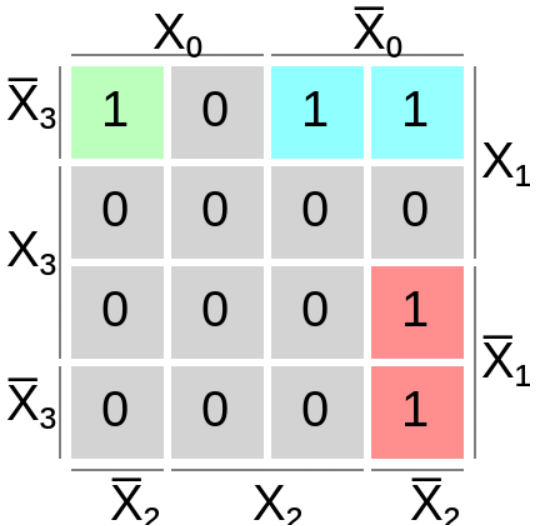
\includegraphics[width=1\linewidth]{course-plis/images/lab1/y3}} а) \\
		\end{minipage}
		\hfill
		\begin{minipage}[h]{0.47\linewidth}
			\center{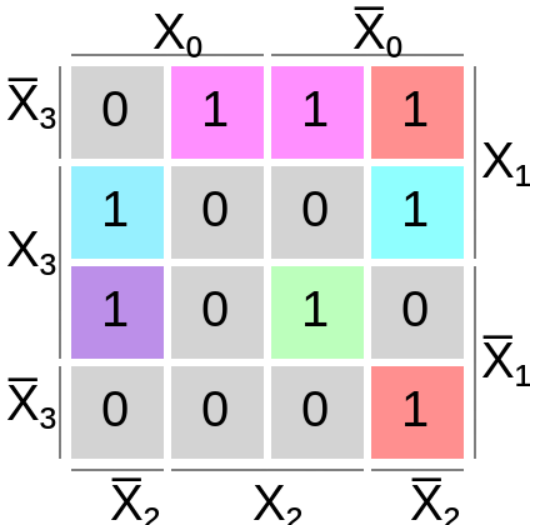
\includegraphics[width=1\linewidth]{course-plis/images/lab1/y2}} \\б)
		\end{minipage}
		\vfill
		\begin{minipage}[h]{0.47\linewidth}
			\center{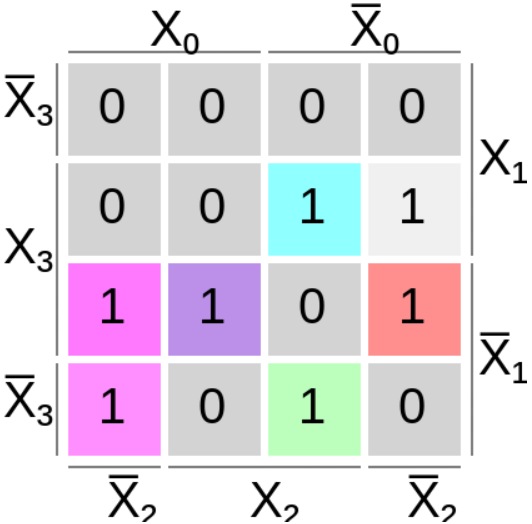
\includegraphics[width=1\linewidth]{course-plis/images/lab1/y1}} в) \\
		\end{minipage}
		\hfill
		\begin{minipage}[h]{0.47\linewidth}
			\center{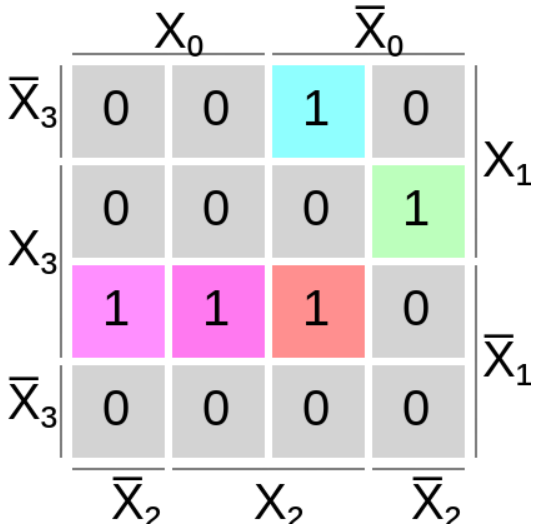
\includegraphics[width=1\linewidth]{course-plis/images/lab1/y0}} г) \\
		\end{minipage}
		\caption{Карты Карно для 4-х переменных для функций а)$Q_3$, б)$Q_2$, в)$Q_2$, г)$Q_1$, д)$Q_0$}
		\label{ris:karno-maps}
	\end{figure}

\section{Минимизация булевых функций}
По построенным картам Карно были описаны {МДНФ} для реализации данных функций на вентильном уровне в редакторе Schematic editor САПР Xilinx ISE Design Suite.

\begin{align}
Q_3 &= \bar{X_3}\bar{X_2}\bar{X_1} \vee  X_2 \bar{X_1}\bar{X_0}  \vee \bar{X_3} X_2\bar{X_0} \\
Q_2 &= \bar{X_3} \bar{X_1} \bar{X_0} \vee \bar{X_3} \bar{X_2} X_1 X_0 \vee X_2  \bar{X_1}  X_0 \vee X_2  X_1  \bar{X_0} \vee  X_3  \bar{X_1}  X_0 \\
Q_1 &=  \bar{X_3}\bar{X_1}X_0    \vee  \bar{X_3} \bar{X_2} X_1 \bar{X_0} \vee     \bar{X_3} X_2  X_0  \vee  X_3 \bar{X_2} \bar{X_1}   \vee  X_3 \bar{X_2} X_0 \\
Q_0 &= \bar{X_2} X_1 X_0 \vee \bar{X_3} X_2 \bar{X_1} X_0 \vee \bar{X_3} X_2 X_1 \bar{X_0} \vee X_3 \bar{X_2} X_0
\end{align}

Также были описаны {МКНФ} для реализации булевых функций средствами VHDL в САПР Xilinx ISE Design Suite.
\begin{align}
Q_3 &=\left(
\bar{X_3}\vee \bar{X_1}
\right) 
\cdot 
\left(
X_2\vee \bar{X_1}
\right) 
\cdot  
\left(
\bar{X_2}\vee \bar{X_0}
\right) \\
Q_2 &= \left(
X_2 \vee X_2 \vee X_1 \vee \bar{X_0}
\right) 
\cdot 
\left( 
\bar{X_3} \vee X_2 \bar{X_1}
\right) 
\cdot 
\left(
X_2 \vee  \bar{X_1} \vee X_0
\right)
\cdot \\
& \left(
\bar{X_2}  \vee \bar{X_1} \vee \bar{X_0}
\right)
\cdot 
\left(\bar{X_3} \vee X_1 \vee X_0
\right)\\
Q_1 & = \left( X_3 \vee X_1 \vee X_0 \right) \cdot
\left( \bar{X_3} \vee \bar{X_1 X_0} \right) \cdot
\left( \bar{X_3} \vee \bar{X_2} \right) \cdot \\
& \left(X_3 \vee X_2 \vee \bar{X_1} \vee \bar{X_0}\right) \cdot
\left(\bar{X_2} \vee X_0\right)\\
Q_0 & = \left( X_3 \vee X_2 \vee X_1 \right) \cdot
\left(  X_2 \vee X_0 \right) \cdot
\left( X_1 \vee X_0  \right) \cdot
\left( \bar{X_3} \vee \bar{X_2} \right) \cdot
\left( \bar{X_2} \vee \bar{X_1} \vee \bar{X_0} \right)
\end{align}


\section{Реализация функций в схемотехническом редакторе}
Были описаны функции $Q_3$,  $Q_2$, $Q_1$,  $Q_0$ на вентильном уровне в схемотехническом редакторе Schematic editor САПР Xilinx ISE Design Suite (см. Рисунок~\ref{fig:circ-editor}).

\begin{figure}[h!]
	%\hfill
	\begin{minipage}[h]{0.47\linewidth}
		\center{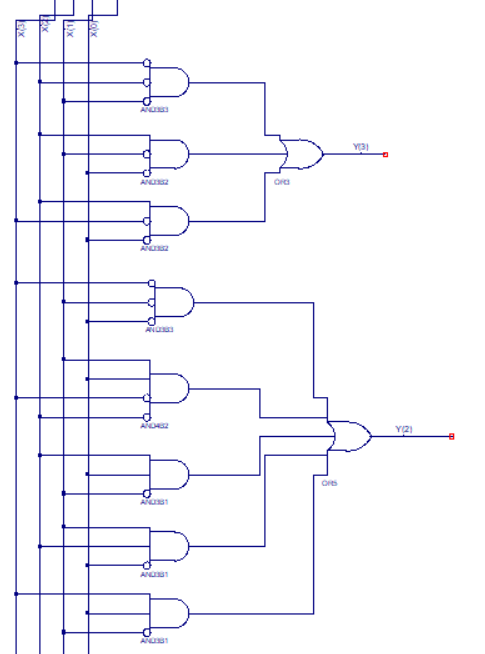
\includegraphics[width=\linewidth]{course-plis/images/lab1/sheme1}} а) \\
	\end{minipage}
	\hfill
	\begin{minipage}[h]{0.47\linewidth}
		\center{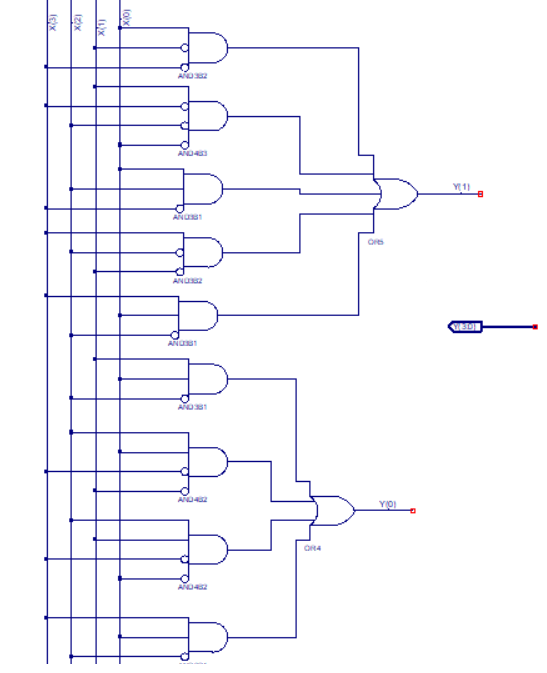
\includegraphics[width=\linewidth]{course-plis/images/lab1/sheme2}} б) \\
	\end{minipage}
	\caption{Схемотехнический редактор а) Лист 1, б) Лист 2}
	\label{fig:circ-editor}
\end{figure}


\newpage
\section{Реализация функций на вентильном уровне}
На основании МКНФ были описаны функции $Q_3$,  $Q_2$, $Q_1$,  $Q_0$ на вентильном уровне c помощью языка Verilog.

Исходный код данного модуля приведен в Приложении~\ref{cha:appendix1} на Листинге~\ref{lst:1mknf}.

%\lstinputlisting{/home/denilai/Documents/repos/latex/scripts/mknf.v}

%\newpage
\section{Реализация функций на поведенческом уровне}
На основании построенной ранее Таблицы истинности~\ref{tab:func-table} были описаны функции $Q_3$,  $Q_2$, $Q_1$,  $Q_0$ на поведенческом уровне c помощью языка Verilog.

Исходный код данного модуля приведен в Приложении~\ref{cha:appendix1} на Листинге~\ref{lst:1beh}.
%\lstinputlisting{/home/denilai/Documents/repos/latex/scripts/behaviour.v}

%\newpage
\section{Создание проекта САПР Xilinx ISE}

Был создан файл верхнего уровня проекта САПР Xilinx ISE Design Suite.
Исходный код данного модуля приведен в Приложении~\ref{cha:appendix1} на Листинге~\ref{lst:1top}.
%\lstinputlisting{/home/denilai/Documents/repos/latex/scripts/top.v}


\section{Тестирование и отладка средствами симулятора iSim}
После компоновки проекта, подключения модуля верхнего уровня, была проведена верификация спроектированных моделей с помощью симулятора iSim из состава САПР Xilinx ISE Design Suite. Результаты тестирования можно видеть в Приложении~\ref{cha:appendix2} на Рисунке~\ref{fig:1isim}.

%% TODO: \usepackage{graphicx} required
%\begin{figure}[htpb]
%	\centering
%	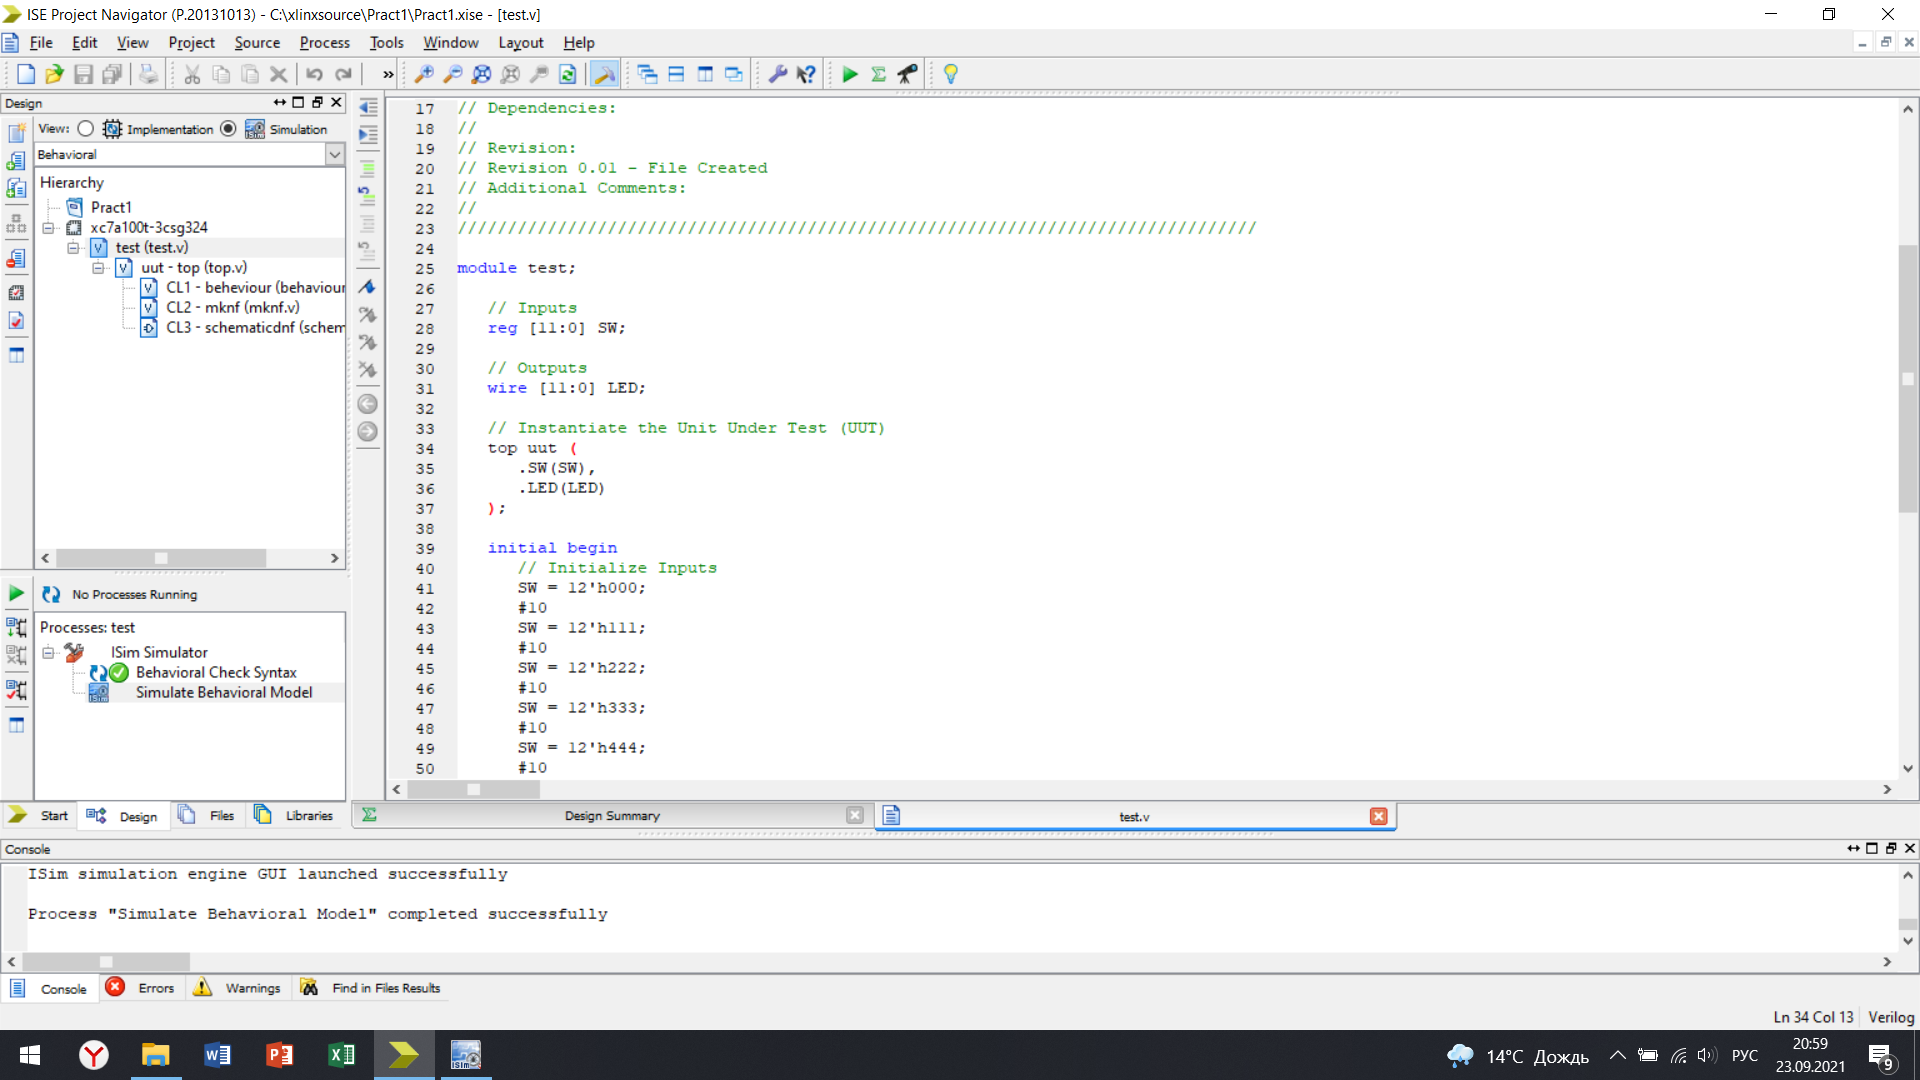
\includegraphics[width=\linewidth]{course-plis/images/lab1/test-result}
%	\caption{Проверка синтаксиса}
%	\label{fig:test-result}
%\end{figure}
%% TODO: \usepackage{graphicx} required
%\begin{figure}[htpb]
%	\centering
%	\includegraphics[width=\linewidth]{course-plis/images/lab1/isim}
%	\caption{Вывод iSim }
%	\label{fig:isim}
%\end{figure}

%\newpage
\section{Вывод}
В данном разделе нами были получены общие навыки работы с программным обеспечением Xilinx ISE Design Suite, изучены основы языка Verilog. С помощью полученных знаний была спроектированы синтезируемые модели комбинационной схемы 4х4, описанной тремя различными способами.

%
%\cite{1},
%\cite{2},
%\cite{3},
%\cite{4},
%\cite{5},
%\cite{6},
%\cite{7},
%\cite{8},
%\cite{9},\\
%\cite{10}\\
